\newpage
\section{Extensions}
Both possible ways for extending Wave have been explored in this work. Gadgets have been implemented with the Wave Gadgets API, and robots with the Java version of the robots API.
\begin{figure}[h]
  \center
    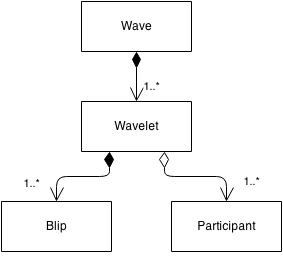
\includegraphics[keepaspectratio, scale=0.75]{Media/Diagrams/Wave/Structure.png}
  \caption{Wave Structure}
  \label{fig:wave_structure}
\end{figure}
To understand where these extensions live, it is necessary to understand how wave is structured. In Figure \ref{fig:wave_structure} you can see how Wave documents are structured. The outermost layer is the wave, a thread or conversation, the whole picture of a conversation. Users are invited to the wave, letting them participate in any of the inner wavelets, when they then become participants. As of today, in current versions of Wave In A Box and Kune, there is only one wavelet inside every wave, but the Wave Protocol allows for multiple wavelets. Blips are individual messages created by a participant, and edited by participants later. Blips have hierarchical structure and can be nested inside other blips. Blips also contain a document in XML-like format, which is the text itself plus all the variations that Wave supports.
\section{Gadgets}
Gadgets are inserted inside a document, together with the content itself. They are placed inside a blip, but belong to the wave and therefore have access to the wave's content, wich is given access by the Gadgets API. But that access is very limited, almost only to access what is called the wave's state, a key-value dictionary that keeps track of every state change that occurs inside the wave.\\[.2cm]
There is actually two differentiated kind of states in a wave:
\begin{itemize}
  \item Private State: Stores information that can only be accessed and modified from the participant that created it. Useful to keep stored private information that is not intended to be shared.
  \item Shared State: Stores the global state of every gadget in this wave, representing the whole picture. Useful for communicating with the other participants and collaborating or comunicating in the gadget.
\end{itemize}
It is important to know that the state belongs to the wave, so gadgets will have access to the other gadgets state, even different instances of the same gadgets. It is then good practice to adopt a system similar to namespaces in programming languages, appending an identifier of the gadget before the key in a way we are not altering or reading an unintended state.\\[.2cm]
Each actual instance of the gadget in a participant's browser is local, variables are not shared between different participants. When a user triggers a state change in his local instance of the gadget, the only thing that can be communicated outside of the browser is a delta, that is an addition, deletion or modification in the key-value pairs that represent the state. This delta is then communicated to the local instance of the gadget in every client's browser so they can act accordingly and represent the new state. That behaviour can be seen represented in figure \ref{fig:wave_state}.
\begin{figure}[H]
  \center
    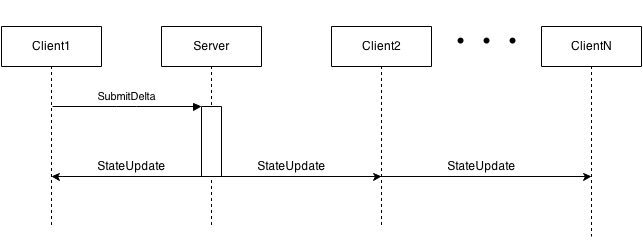
\includegraphics[keepaspectratio, scale=0.6]{Media/Diagrams/Wave/StateSequence.png}
  \caption{Wave state transmission}
  \label{fig:wave_state}
\end{figure}
The Gadgets API asks you to follow a class hierarchy in order to be able to correctly communicate with wave. That hierarchy is as seen in Figure \ref{fig:gadget_classes}.\\[.2cm]
\begin{figure}[h]
  \center
    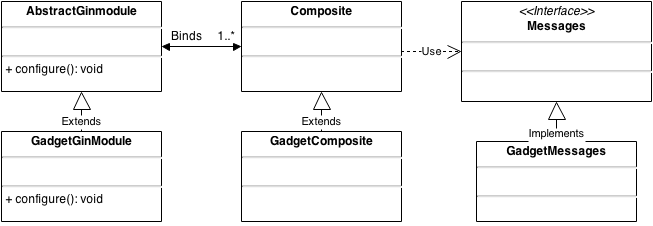
\includegraphics[keepaspectratio, scale=0.5]{Media/Diagrams/Gadget/Gadget.png}
  \caption{Gadgets API class structure}
  \label{fig:gadget_classes}
\end{figure}
Those classes will interact in the following way:
\begin{itemize}
  \item AbstractGinModule: GIN is Guice for GWT client-side code, built on top of Guice and with a subset of Guice binding language. It allows the programmer to follow the pattern of dependency injection. This module attaches all of the modules together.
  \item Composite: Is the actual visual representation of the gadget. This is a GWT class ideated for creating custom widgets. Composites can contain a panel, and inside the panel comples GWT component hierarchies can be built. All features of GWT are supported thanks to this component.
  \item Messages: A GWT interface meant to be implemented by a class that gives access to the strings needed to build the interface. Those strings can be localized to make the gadget available in different languages for each client. The locale is determined by the Accept-Language field in the browser's HTTP request \cite{ref:gwt_internationalization} and served at runtime to the browser. Typically this class will be used from the Composite, or any of its inner components, to fill them with human-readable language.
\end{itemize}
With every one of the gadgets there is available a tester and a deployer, both of them depending on the main gadget, which is common for both.
\begin{figure}[H]
  \center
    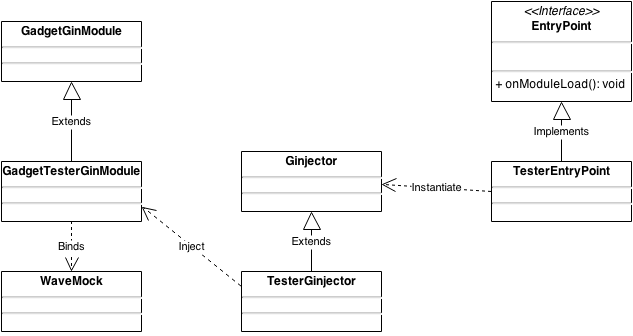
\includegraphics[keepaspectratio, scale=0.5]{Media/Diagrams/Gadget/Tester.png}
  \caption{Gadget Tester Structure}
  \label{fig:gadget_tester}
\end{figure}
The tester project seen in Figure \ref{fig:gadget_tester} shows the common class hierarchy used in every one of the tester projects, which makes use of the development mode available in GWT, so gadgets can be quickly tested before deploying them. It is linked to the one seen in Figure \ref{fig:gadget_classes} by the GadgetGinModule, whis is inherited by the GadgetTesterGinModule. This new Gin module adds another injection, the WaveMock. This is a mock class that simulates the basics of the behaviour of the Wave infrastructure without the need to deploy the whole Wave system. To complete the needs of GIN a class extending Ginjector is created, the TesterGinjector, whose task is to actually inject the GinModule. This injector is instantiated inside a class that implements the interface EntryPoint that, as its name says, will be the entry point of out gadget in the onModuleLoad method. This project has to be run as a Web Application with Google's App Engine.
\begin{figure}[H]
  \center
    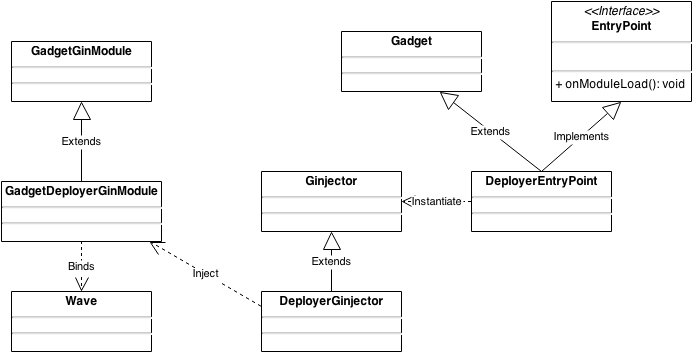
\includegraphics[keepaspectratio, scale=0.5]{Media/Diagrams/Gadget/Deployer.png}
  \caption{Gadget Deployer Structure}
  \label{fig:gadget_deployer}
\end{figure}
The deployer project represented in Figure \ref{fig:gadget_deployer} is the project used to generate all the final JavaScript files ready to deploy to a web server with support for gadgets. An intermediate XML file containing JavaScript code is generated with enough logic to figure out which one of the browser and locale configuration has to be served.\\[.2cm]
It is very similar to the tester organization but with two basic differences. First, the GadgetGinModule now binds the class Wave instead of a Wave mock, as it will be running in the whole Wave environment. The other difference is that the EntryPont, as well as implementing the same interface as before, now also extends the Gadget class, coming from the Gadgets API and representing a gadget. This project needs to be GWT compiled to succesfully generate all the files.\\[.2cm]
Gadgets have been tested for deployment using tomcat as a web server and shindig as a gadgets server with support for opensocial. Several files are generated after GWT compiling, and they should all be put together in the same directory and accessible from the outside. Shindig is then deployed as an application inside tomcat.\\[.2cm]
Shindig needs to be configured accordingly:
\begin{itemize}
  \item First add ``wave'' to the gadgets.container in the \verb|container.js| file, in order to support Wave. As Wave does not use security token (OAuth's authentication token) for gadgets, you have to set Shindig not to require it by adding the following line: \verb|``render_token_required'' : false,|.
  \item Then you have to instruct Wave to use the gadgets server that was configured. The place to do that is a file called server.config in Wave In A Box, and wave-server.properties in Kune. Set the properties \verb|gadget_server_hostname| to the host running Shindig, and \verb|gadget_server_port| to the port where it is running.
\end{itemize}

\subsection{Creative Commons Gadget}

\subsubsection{Introduction}
The default license for any creation of any kind is the restrictive copyright. Copyright tries to ensure that all the rights remain to the original author of the content, but sometimes it can be advantageous to let people freely or semi-freely use, distribute or modify the content. One of the most popular, with over 400 million \cite{ref:the_power_of_open}, are the Creative Commons set of licenses. These are not adecuate for licensing software, but in the context of Wave the content is usually creative work, for which Creative Commons makes a good job.

\subsubsection{State of the Art}
Wave doesnt have any way of publishing your content under any specific license. Kune has the option for publishing Waves in your personal space under one of the existing Creative Commons Licenses. Outside of the personal space, Kune preserves Wave's aspect and removes the space where the license is in the personal space, so no license is imposed to other participants in a wave.

\subsubsection{Results}
This extension allows participants to set a Creative Commons license to a specific blip, by inserting a gadget in the content and answering questions to reach the adequate license that meets the requierements. The Figure \ref{fig:cc_gadget} shows the final result of this extension.

\begin{figure}[h]
  \center
    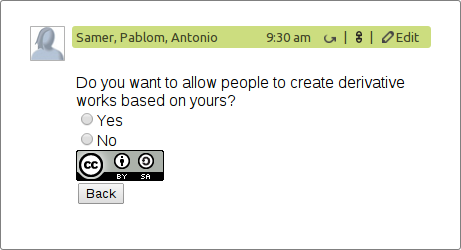
\includegraphics[keepaspectratio, scale=0.7]{Media/Captures/Extensions/CCGadget.png}
  \caption{Creative Commons Gadget}
  \label{fig:cc_gadget}
\end{figure}


\thispagestyle{sectioned}
\chapter{Pollymer}
%\addcontentsline{toc}{chapter}{\numberline{Decision Maker Gadget}}
When talking in a group of people it is sometimes necessary to take a decision about a specific aspect. The easiest way to achieve this is by talking, and Wave with real time communication and editing common documents makes this easy. But this way it might be difficult to easily differentiate all the different options, see who agrees with each one of the options, or quickly decide one. This extension allows every participant to \textbf{choose an option or add new options to the decision}. Participants are also able to quickly see who voted each option along with their user avatar images. This features accompanied by Wave's style of communication make consensus and decision making easier.

\label{subsec:decision_soa}
\section{State of the Art}
Because of the nature of Wave, decision making is a very important and basic, so there has been several gadgets made regarding that. It also easily explores all the basic possibilities that the Gadgets API provides. Figures \ref{fig:poll} and \ref{fig:consensuall} show two of them: The first one is Poll by Eric Williams, focused on showing statistics about the results, maybe useful when there is a high amount of votes. The second one is Consensuall \cite{ref:consensuall} by Antonio Tenorio, focused on sharing the personal opinion of each voter about an issue and reaching consensus on it.\\[.2cm]
\begin{figure}[h]
  \center
    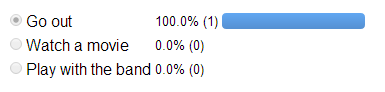
\includegraphics[keepaspectratio, scale=0.7]{Media/Captures/Extensions/DecisionGadgets/other.png}
  \caption{Poll}
  \label{fig:poll}
\end{figure}
\begin{figure}[h]
  \center    
    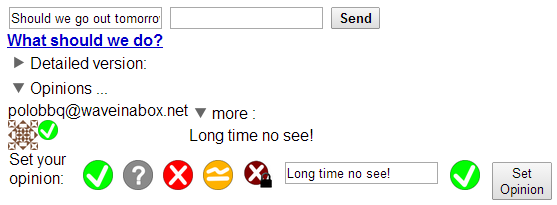
\includegraphics[keepaspectratio, scale=0.7]{Media/Captures/Extensions/DecisionGadgets/consensuall.png}
  \caption{Consensuall}
  \label{fig:consensuall}
\end{figure}
Pollymer falls in between both of them by letting people add their own answers, see a representation of the votes and who personally voted for each.

\section{Results}
Pollymer is a gadget that can be inserted anywhere in a blip. A title is chosen for the issue at hand, and then \textbf{different options} answering that title can be inserted by anyone who sees the gadget, not only the creator. One of the decisions can be instantly chosen by clicking on it.
\begin{figure}[h]
  \center
    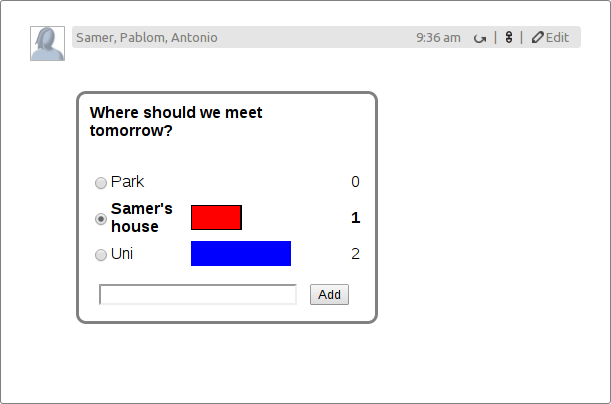
\includegraphics[keepaspectratio, scale=0.35]{Media/Captures/Extensions/DecisionMakerGadget.png}
  \caption{Pollymer}
  \label{fig:decision_maker_gadget}
\end{figure}
When there have been decisions chosen by different participants, \textbf{hovering the mouse over} the number of votes on the right will show the names and pictures of the participants that voted for it, as represented in Figure \ref{fig:decision_maker_votes}. Names and pictures are taken from their Wave profile.
\begin{figure}[h]
  \center
    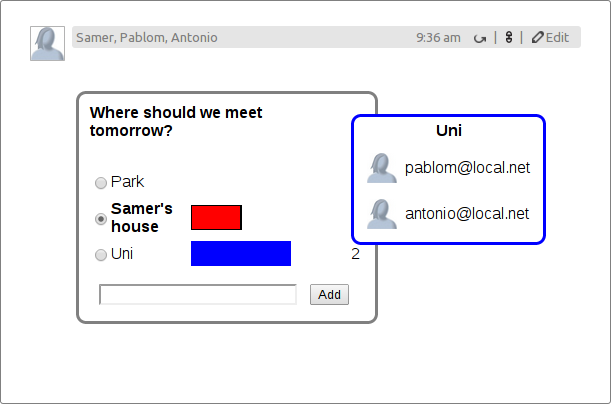
\includegraphics[keepaspectratio, scale=0.35]{Media/Captures/Extensions/DecisionMakerGadget_votes.png}
  \caption{Pollymer Voters}
  \label{fig:decision_maker_votes}
\end{figure}
This gadget also relates to the structure shown in Figure \ref{fig:gadget_classes}. The GinModule is the DecisionMakerGinModule, the Composite is the DecisionMakerMainPanel, and the Messages class is represented by the class DecisionMakerMessages. This gadget is slightly more complex than the Creative Commons one, so the class diagram with its specifics is shown in Figure \ref{fig:decision_maker_diagram}.
\begin{figure}[h]
  \center
    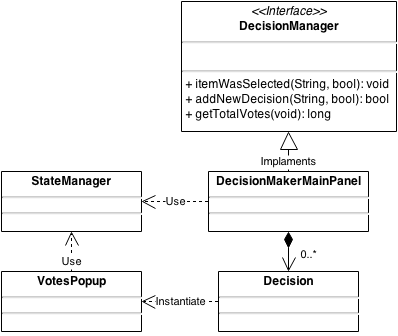
\includegraphics[keepaspectratio, scale=0.5]{Media/Diagrams/Gadget/DecisionMaker.png}
  \caption{UML Class Diagram, Pollymer}
  \label{fig:decision_maker_diagram}
\end{figure}
The interface DecisionManager is extended. It is meant to represent all that can be done with the decisions: select one, add a new decision, and get the total votes of one specific decision. The DecisionMakerMainPanel implements it, and is also the container for all the decisions. A decision represents one of the options that can be chosen, and generates the Popup showing who voted for it. A StateManager is also used to handle everything related to the Wave's state.\\[.2cm]
There are three different types of entries in the Wave's state:
\begin{itemize}
  \item \textbf{Count of votes}: There is one entry of this kind for each decision. To identify which decision this entry is for, the title of the decision is stored as a key. Therefore, the decision titles have to be unique. The value of this entry is the amount of votes that decision has, making it quick to retrieve the amount and show the vote count.
  \item \textbf{Voters}: Again, one entry for each decision and the title of the decision as an unique identifier. The value is a list of all the people that voted for that decision. As the state is only able to store a string, the list is like \verb+|user1@kune.cc|user2@kune.cc|user3@kune.cc|+. This entry is used to know if a particular user has voted for a decision, and to fill the information inside the votes popup.
  \item \textbf{Title}: There is one single entry for each gadget. The value of this entry is the name of the decision to be taken. Used to fill the title after it has been set.
\end{itemize}
\section{Conclusions and Future Work}
There are already several alternatives for decision making, each one with their unique way of doing things, and there is certainly already one suitable for every need, and Pollymer doesn't innovate in almost any aspect. This alternative has limitations though: There is no option for multi-choice answers, no way of editing the title after being created, and the list of votes can get a little uncomfortable to see after a large amount of votes has been made. Multi-choice answers would put this gadget \textbf{closer to a consensus tool}, and being able to block options would make the divergence among opinions more visible.
\newpage

\thispagestyle{sectioned}
\chapter{AppearWOW}
\label{subsec:video_intro}
%\addcontentsline{toc}{chapter}{\numberline{Video Conference Gadget}}
From D1.3 Design Guidelines (Section Technical Features) \cite{ref:p2pvalue}: ``The platform should therefore include tools for collaboration, including key features, such as: Synchronous communication with video and voice communication''.\\[.2cm]
Wave is meant for text communication. Text has the advantage that it can be stored easily, searched later and edited simultaneously, but lacks the naturality of human-to-human interaction. To get as close as possible to it we need voice and video. Then collaborating on text can be made more efficiently. This gadget makes it possible to \textbf{speak to up to 16 other users and see them}.

\section{State of the Art}
\label{subsec:video_soa}
There is no alternative to video or audio communication integrated on Wave. There is other alternatives though outside of it, some of them shown in Figure \ref{fig:skype_hangouts}.
\begin{figure}[h]
  \center
    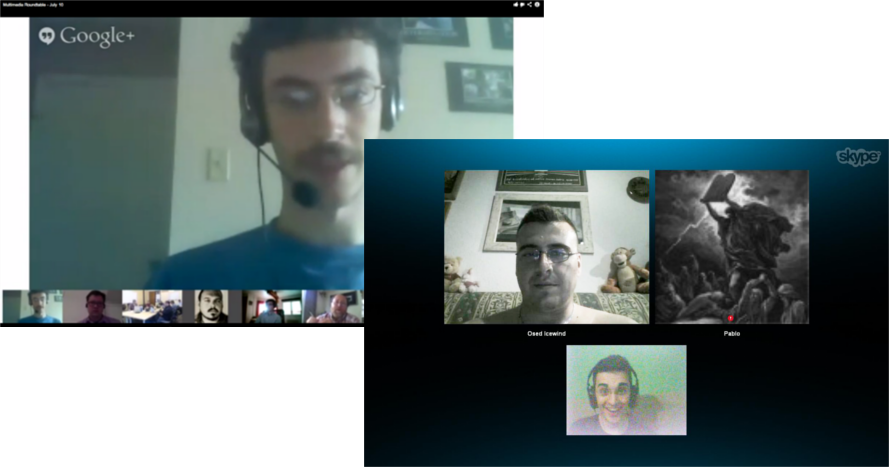
\includegraphics[keepaspectratio, scale=0.43]{Media/Captures/Soa/skype_hangouts.png}
  \caption{Hangouts and Skype}
  \label{fig:skype_hangouts}
\end{figure}
They focus on video, even hiding text communication to leave more room to the video. AppearWOW can be mixed with text above and below, leaving the video communication as an addition and not the main point. Both video communication tools shown (Google's Hangouts and Microsoft's Skype) require you to have a specific user account to use their services, while this gadget lets you join the \textbf{video communication from within Wave}, but also from an external link without giving any kind of personal information.

\section{Results}
To make this gadget it has been essential the use of a pre-existing service called \textbf{appear.in} \cite{ref:appearin}. They provide the whole video and audio communication based on WebRTC \cite{ref:webrtc}, and also facilitate an easy way to use their service in an external website. It is a JavaScript component that can be put inside an iframe, and it will take care of almost everything. Figure \ref{fig:video_gadget} shows the final result of this integration.
\begin{figure}[h]
  \center
    
\includegraphics[keepaspectratio, scale=0.8]{Media/Captures/Extensions/VideoGadget/RoomSelection.png}
  \caption{Room Selection Screen}
  \label{fig:video_gadget_room}
\end{figure}
When a user inserts the gadget, he will be prompted with the room selection screen shown in Figure \ref{fig:video_gadget_room}, letting him choose the identifier of the room people will meet in. The same room can be visited from different waves, and also directly from appear.in, as room names can not be duplicated.
\begin{figure}[h]
  \center
    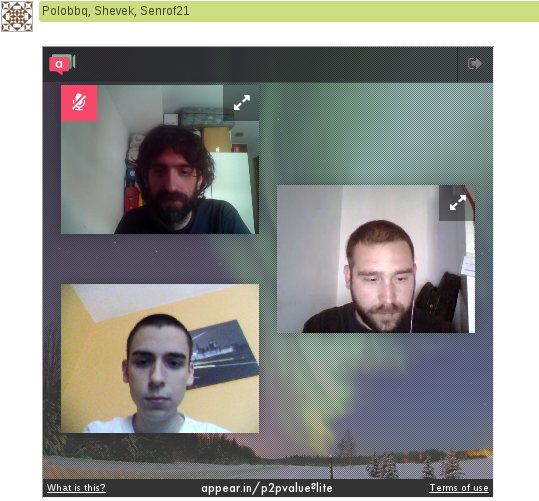
\includegraphics[keepaspectratio, scale=0.45]{Media/Captures/Extensions/VideoGadget.png}
  \caption{Video Conference Gadget}
  \label{fig:video_gadget}
\end{figure}
It was shown in Figure \ref{fig:gadget_classes} the basic structure of a gadget. The composite is represented by the VideoGadgetMainPanel, the Messages are the class VideoGadgetMessages, and the GinModule is realized by VideoGadgetGinModule. Outside from that, the structure is relatively simple.\\[.2cm]
As appar.in is a JavaScript service, multiple calls to \textbf{native JavaScript} have been made inside this gadget.
The service appear.in uses the name of the room as a unique identifier, so the gadget asks the user for a name before entering the room. The gadget also makes use of appear.in's \verb|?lite| feature, that simplifies the user interface, leaving more space for the images of the video. The \textbf{camera is accessed through the browser}, so no additional software has to be installed.\\[.2cm]
The Wave state in this gadget is really simple, the only thing stored in it is the name of the room to enter it directly if it has already been set.\\[.2cm]
\begin{figure}[h]
  \center
    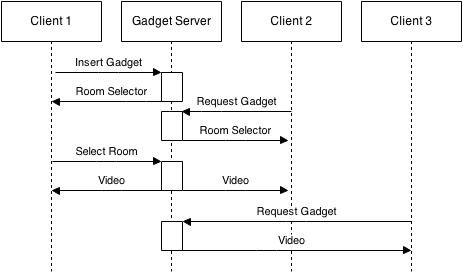
\includegraphics[keepaspectratio, scale=0.6]{Media/Diagrams/Gadget/VideoSequence.png}
  \caption{UML Sequence Diagram, AppearWOW}
  \label{fig:video_gadget_sequence}
\end{figure}
Figure \ref{fig:video_gadget_sequence} shows how the gadget reacts to requests. Once the gadget is inserted, the room selection screen will be shown, allowing any participant to select the name of the room the participants will meet in. When a room is selected, the participants automatically enter the room. If another participant joins the wave once the room has been selected, he will be served the video conference directly.
\section{Conclusions and Future Work}
The fact that this extension is completely \textbf{dependant on an external closed-source service} is a big limitation. The service could stop working at any time, technical improvements on video or audio communication can not be made, limitations like the maximum of 16 online users can not be avoided, the way to use it could change making it necessary to update the gadget, and other changes may arise.
\newpage


\section{Robot}
Robots were created in Wave with the intention to be able to act exactly as an actual human participant. Revisiting Figure \ref{fig:wave_structure} we can understand how robots can participate: They are invited to the Wave by inserting their unique identifier. They will aprear as invited without any apparent indication that they are a robot. Robots can make changes to the Wave such as creating a new blip, editing them, changing annotations...\\[.2cm]
In order to be able to interact with Wave it is necessary to register the robot with the Wave server where the robot will be run. For example, for the Kune node kune.cc, go to \url{http://kune.cc/robot/register/create} and you will be prompted with the screen shown in Figure \ref{fig:robot_register}.
\begin{figure}[H]
  \center
    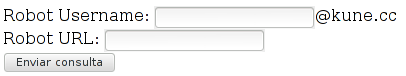
\includegraphics[keepaspectratio, scale=0.6]{Media/Captures/Wave/RegisterRobot.png}
  \caption{Robot Registration Screen}
  \label{fig:robot_register}
\end{figure}
As username set the name you wish to give your robot, it should be a free name in the server, as names are unique. In the URL enter the URL where the gadget will be launched, it should be an URL reachable from within the Wave server. After sending the data you will receive a Consumer Token matching the name you entered, and a Consumer Token Secret: a secret key you will need to use to authenticate with OAuth and guarantee the identity of your robot.\\[.2cm]
There is no equivalent to the tester mode from GWT, but running a server for the robots is easy enough so it is not a hassle. Using Maven plus Jetty you can set the Maven goal to \verb|jetty:run| and the robot will be run.\\[.2cm]
Robots do basically two thins: Act when needed, and react to events. Acting means modifying the documents, creating new blips... And receiving events means a callback will be made to the robot when something from an external action happens on the Wave. The kind of events that are notified to the robot are the following:
\begin{itemize}
  \item WaveletBlipCreated: Triggered when a new blip is created.
  \item WaveletBlipRemoved: Triggered when a blip is deleted.
  \item WaveletParticipantsChanged: Triggered when a participant is added or removed.
  \item WaveletSelfAdded: Triggered when the own robot is added as a participant.
  \item WaveletSelfRemoved: Triggered when the own robot is removed as a participant.
  \item DocumentChanged: Triggered when the text of a document changes.
  \item AnnotatedTextChanged: Triggered when the annotations of a document change.
\end{itemize}
There are other events documented such as GadgetStateChanged or WaveletTagsChanged, which even though available through the Robots API will not be triggered on the server, and therefore never received.

\subsection{Colorizer Robot}
Again, text communications gets in the way of collaboration in some aspects. When working between several people it is sometimes necessary to talk about some aspect of the work they disagree in. In plain text, when there are more than two collaborators, there is no way to know who edited what, so those kind of issues can't be addressed personally. A robot is needed in order to know when and what changes are being made.

\subsubsection{State of the Art}
In Wave it is possible to see who has participated in a blip as shown in Figure \ref{fig:participants}, but it is not possible to see exactly what that participant has modified what part of the document.
\begin{figure}[H]
  \center
    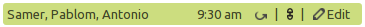
\includegraphics[keepaspectratio, scale=0.7]{Media/Captures/Wave/Participants.png}
  \caption{Blip Participants in Kune}
  \label{fig:participants}
\end{figure}
The other thing Wave does to try to keep people informed on when changes happen, is to highlight the changes that just happened and write the author's name next to it, as shown in Figure \ref{fig:participants2}. The problem is it is not permanent, so you only realize of the change if you were already looking at the content being changed.
\begin{figure}[H]
  \center
    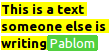
\includegraphics[keepaspectratio, scale=0.7]{Media/Captures/Wave/Participants2.png}
  \caption{Change Highlighting in Kune}
  \label{fig:participants2}
\end{figure}
Also, this extension is heavily inspired in Pads, services like PiratePad, Etherpad, TitanPad and many others, that offer an online collaboration tool that allows to concurrently write plain-text documents. They show a specific color for each participant to quickly see who edited what. TitanPad in Figure \ref{fig:titanpad}, even though not the only, has the capability to show a timeline and revisit past states of the Pad, so no information is lost even after being modified.
\begin{figure}[h]
  \center
    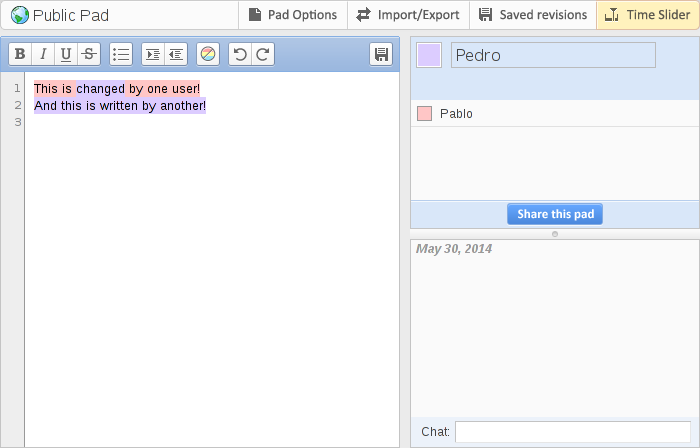
\includegraphics[keepaspectratio, scale=0.4]{Media/Captures/Soa/TitanPad.png}
  \caption{TitanPad}
  \label{fig:titanpad}
\end{figure}

\subsubsection{Results}
This extension, in the shape of a robot, goes around that problem by assigning a color to each participant, and painting the background of the text that participant edits. The result can be seen in Figure \ref{fig:colorizer_editions}. It also keeps track of who has each color and puts it in a blip under the main blip of the wave, as seen in Figure \ref{fig:colorizer_editors}. It is also possible to get around the colorizing of any given blip by starting it with \verb|@Robot clear annotations|, being ``Robot'' the actual name of the robot that it was registered with.\\[.2cm]
\begin{figure}[H]
  \center
    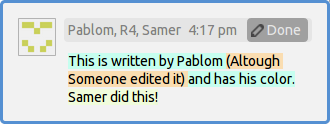
\includegraphics[keepaspectratio, scale=0.8]{Media/Captures/Extensions/Colorizer/ColorizerEditions.png}
  \caption{Colorizer Robot Colors}
  \label{fig:colorizer_editions}
\end{figure}
\begin{figure}[h]
  \center
    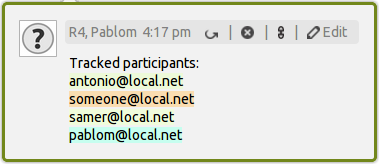
\includegraphics[keepaspectratio, scale=0.7]{Media/Captures/Extensions/Colorizer/ColorizerEditors.png}
  \caption{Colorizer Robot Tracking Participants}
  \label{fig:colorizer_editors}
\end{figure}
The way to make the background of the text be of a specific color is by changing the annotations of the document. Annotations in Wave are tags affecting a range of text and altering its properties, but they don't affect the text itself. Annotations are also able to be transmitted through the Federation Protocol. Every annotation is defined by a name (What it does), a range (What characters of text it affects), and a value (What value should that annotation take on that range). There are annotations for text size, links, language... For this robot specifically the annotation \verb|style/backgroundColor| is the one being set in the changed text.\\[.2cm]
The way to know when the changes happen is by subscribing th the DocumentChanged event explained before. This event will be triggered anytime anyone modifies the text.\\[.2cm]
\begin{figure}[h]
  \center
    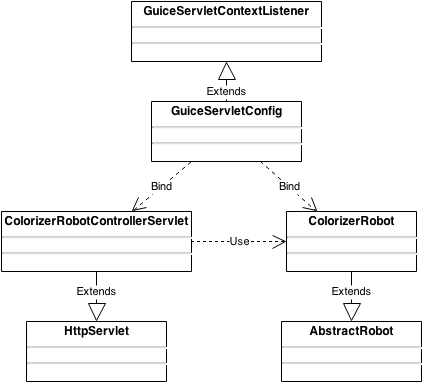
\includegraphics[keepaspectratio, scale=0.5]{Media/Diagrams/Robot/Colorizer.png}
  \caption{Colorizer Robot Class Diagram}
  \label{fig:colorizer_diagram}
\end{figure}
That only leaves one task left: The DocumentChanged event tells us the document has changed, but not what part changed or how it changed, so it is up to us to extract that information. To achieve it Google's google-diff-match-patch, a Java library that is able to extract the difference between two chunks of plain text. Every time the document is changed, the difference with the last version is calculated, and the new content is attributed to the participant that changed it.\\[.2cm]
Figure \ref{fig:colorizer_diagram} represents the class structure of the Colorizer Robot. The HttpServlet is the responsible of receiving the communication from the Wave Protocol. The ColorizerRobot sets up the OAuth authentication with the token received when registering the robot. Also, thanks to the AbstractGadget class it is registered to receive all the events. The GuiceServletConfig binds the necessary dependencies together.\\[.2cm]
This extension, as said before, uses an API for diff that works with plain text. That means changes on annotations are not detected. Also, diff detection can be problematic in some cases. The difference between two documents is always computed correctly, but as the library does not have information on where the text changed, it will sometimes attribute a change to a wrong position of the text. For example: We have the string ``abc'', and a participant decides to add a new ``b'' to the left of the already existing ``b''. The end result would be ``abbc'', where the first apparition of the letter will be the change from the last version of the text. But because of how the diff calculation is made, the library will come up with the result that the difference between those two texts is the ``b'' on the right and the robot will put the background color in the wrong character. This small example can be extrapolated to more complex and problematic cases.

